% !TEX program = pdflatex
% !TEX enableSynctex = true
% !BIB program = bibtex

\documentclass[12pt]{article}

\usepackage{setspace}
\usepackage{amsmath}
\usepackage{amsfonts}
\usepackage{graphicx}
\usepackage{float}
\usepackage{natbib}
\addtolength{\oddsidemargin}{-.7in}
\addtolength{\evensidemargin}{-.7in}
\addtolength{\textwidth}{1.4in}
\usepackage{enumerate}
\onehalfspacing
\usepackage{geometry} % Required for customizing page layout
\usepackage{ragged2e}

\usepackage{caption}
\usepackage{booktabs}

\usepackage{hyperref}
\hypersetup{
	pdfstartview = FitH,
	pdfauthor = {...},
	pdftitle = {...},
	pdfkeywords = {...; ...; ...; ...},
	colorlinks = true,
	linkcolor = blue,
	urlcolor = blue,
	citecolor = blue,
	linktocpage=true
}



\title{\vspace{-0.5cm} Optimal Debt Financing Strategies Under Heterogeneous Debt Contracts}
\author{Barnabás Székely \\ \small  Goethe-Universität Frankfurt, GSEFM}
\date{}


\begin{document}
\maketitle


\subsection*{Introduction} \label{sec:introduction}

Credit market frictions are traditionally characterized in the macro-finance literature as asset-based borrowing constraints. Recent contributions  challenged this approach based on more granular analyses of debt contracts (Lian and Ma, 2021; Dreschel, 2023). They argue that most corporate debt is backed by future cash flows rather than assets; hence, credit frictions are better described as borrowing constraints defined by earnings. This reassessment of credit frictions has had a substantial impact on certain predictions of macro-finance models. However, the incentives to borrow (and lend) against future cash flows are not yet fully explored. This paper fills this gap in the literature and presents some policy recommendations in light of this analysis. 

First, I conduct an empirical analysis of the debt financing strategies of North American corporations. This informs a structural heterogeneous agents model describing the tradeoffs that govern debt financing strategies. Cash flow-based debt contracts allow lenders to extract a portion of a borrower's going-concern value under financial distress. On the flip side, these contracts are not secured by collateral, making them ineffective in recovering the liquidation value of firms. This tradeoff highlights the ex-ante probability of liquidation as an important predictor of borrowing against future cash flows: when lenders expect that the borrower will face liquidation under financial distress, they offer cash flow-backed loans with unfavorable terms, compelling the borrower to choose asset-based debt financing.

Previous contributions focused solely on covariates of liquidation probability, such as size, profitability, and asset specificity. These are relevant determinants in their own right. However, the ex-ante probability of liquidation holds a particular policy relevance. Bankruptcy frameworks are typically perceived as balancing the inefficient liquidation of healthy businesses and the wasteful reorganization of incumbents. Considering CF-based lending changes this arithmetic. If small firms face liquidation under financial distress too frequently, they might find it expensive to obtain cash flow-backed debt - even though they stand to benefit the most from this form of debt finance. This emphasizes the importance of a regulatory environment that supports the reorganization of small firms. I examine the effects of such policies in the structural model.

\subsection*{Empirical analysis of the debt financing strategies}
In the main body of the empirical analysis, I study debt-level data collected from S\&P's Capital IQ, and firm-level data is from Compustat North America. Overall, I study a total of 180388 debt contracts held by 8974 non-financial corporations in the United States and Canada, between 2010Q1 and 2023Q2. Bankruptcy data is collected for the same period, from the Integrated Data Base published by US Federal Judicial Center (FJC). Moreover, I study ORBIS data to extend the cross-country coverage of my analysis. \vspace{3mm} \\
I classify asset-based or cash flow-based based debt contracts manually, following the methodology of Lian and Ma (2021). Out of all debt instruments, 52.4\% can be classified as cash flow-based, collectively representing 75.5\% of the total debt by volume. Figure \ref{chart:CFLcdf} summarizes the firm level distribution of CFL reliance (defined as CF-based debt to total debt). Firms often hold asset-based and CF-based debt simultaneously, which implies that both are available in most cases. Remarkably, when plotted against firm size, average CFL reliance shows a U-shaped pattern, indicating that small corporations also rely heavily on CF-based debt financing. This is robust over time, across sectors, and to different indicators of firm size.

\begin{figure}[H]  % [h] indicates placing the image here
    \centering
    \caption{The distribution of CFL reliance} \label{chart:CFLcdf}
    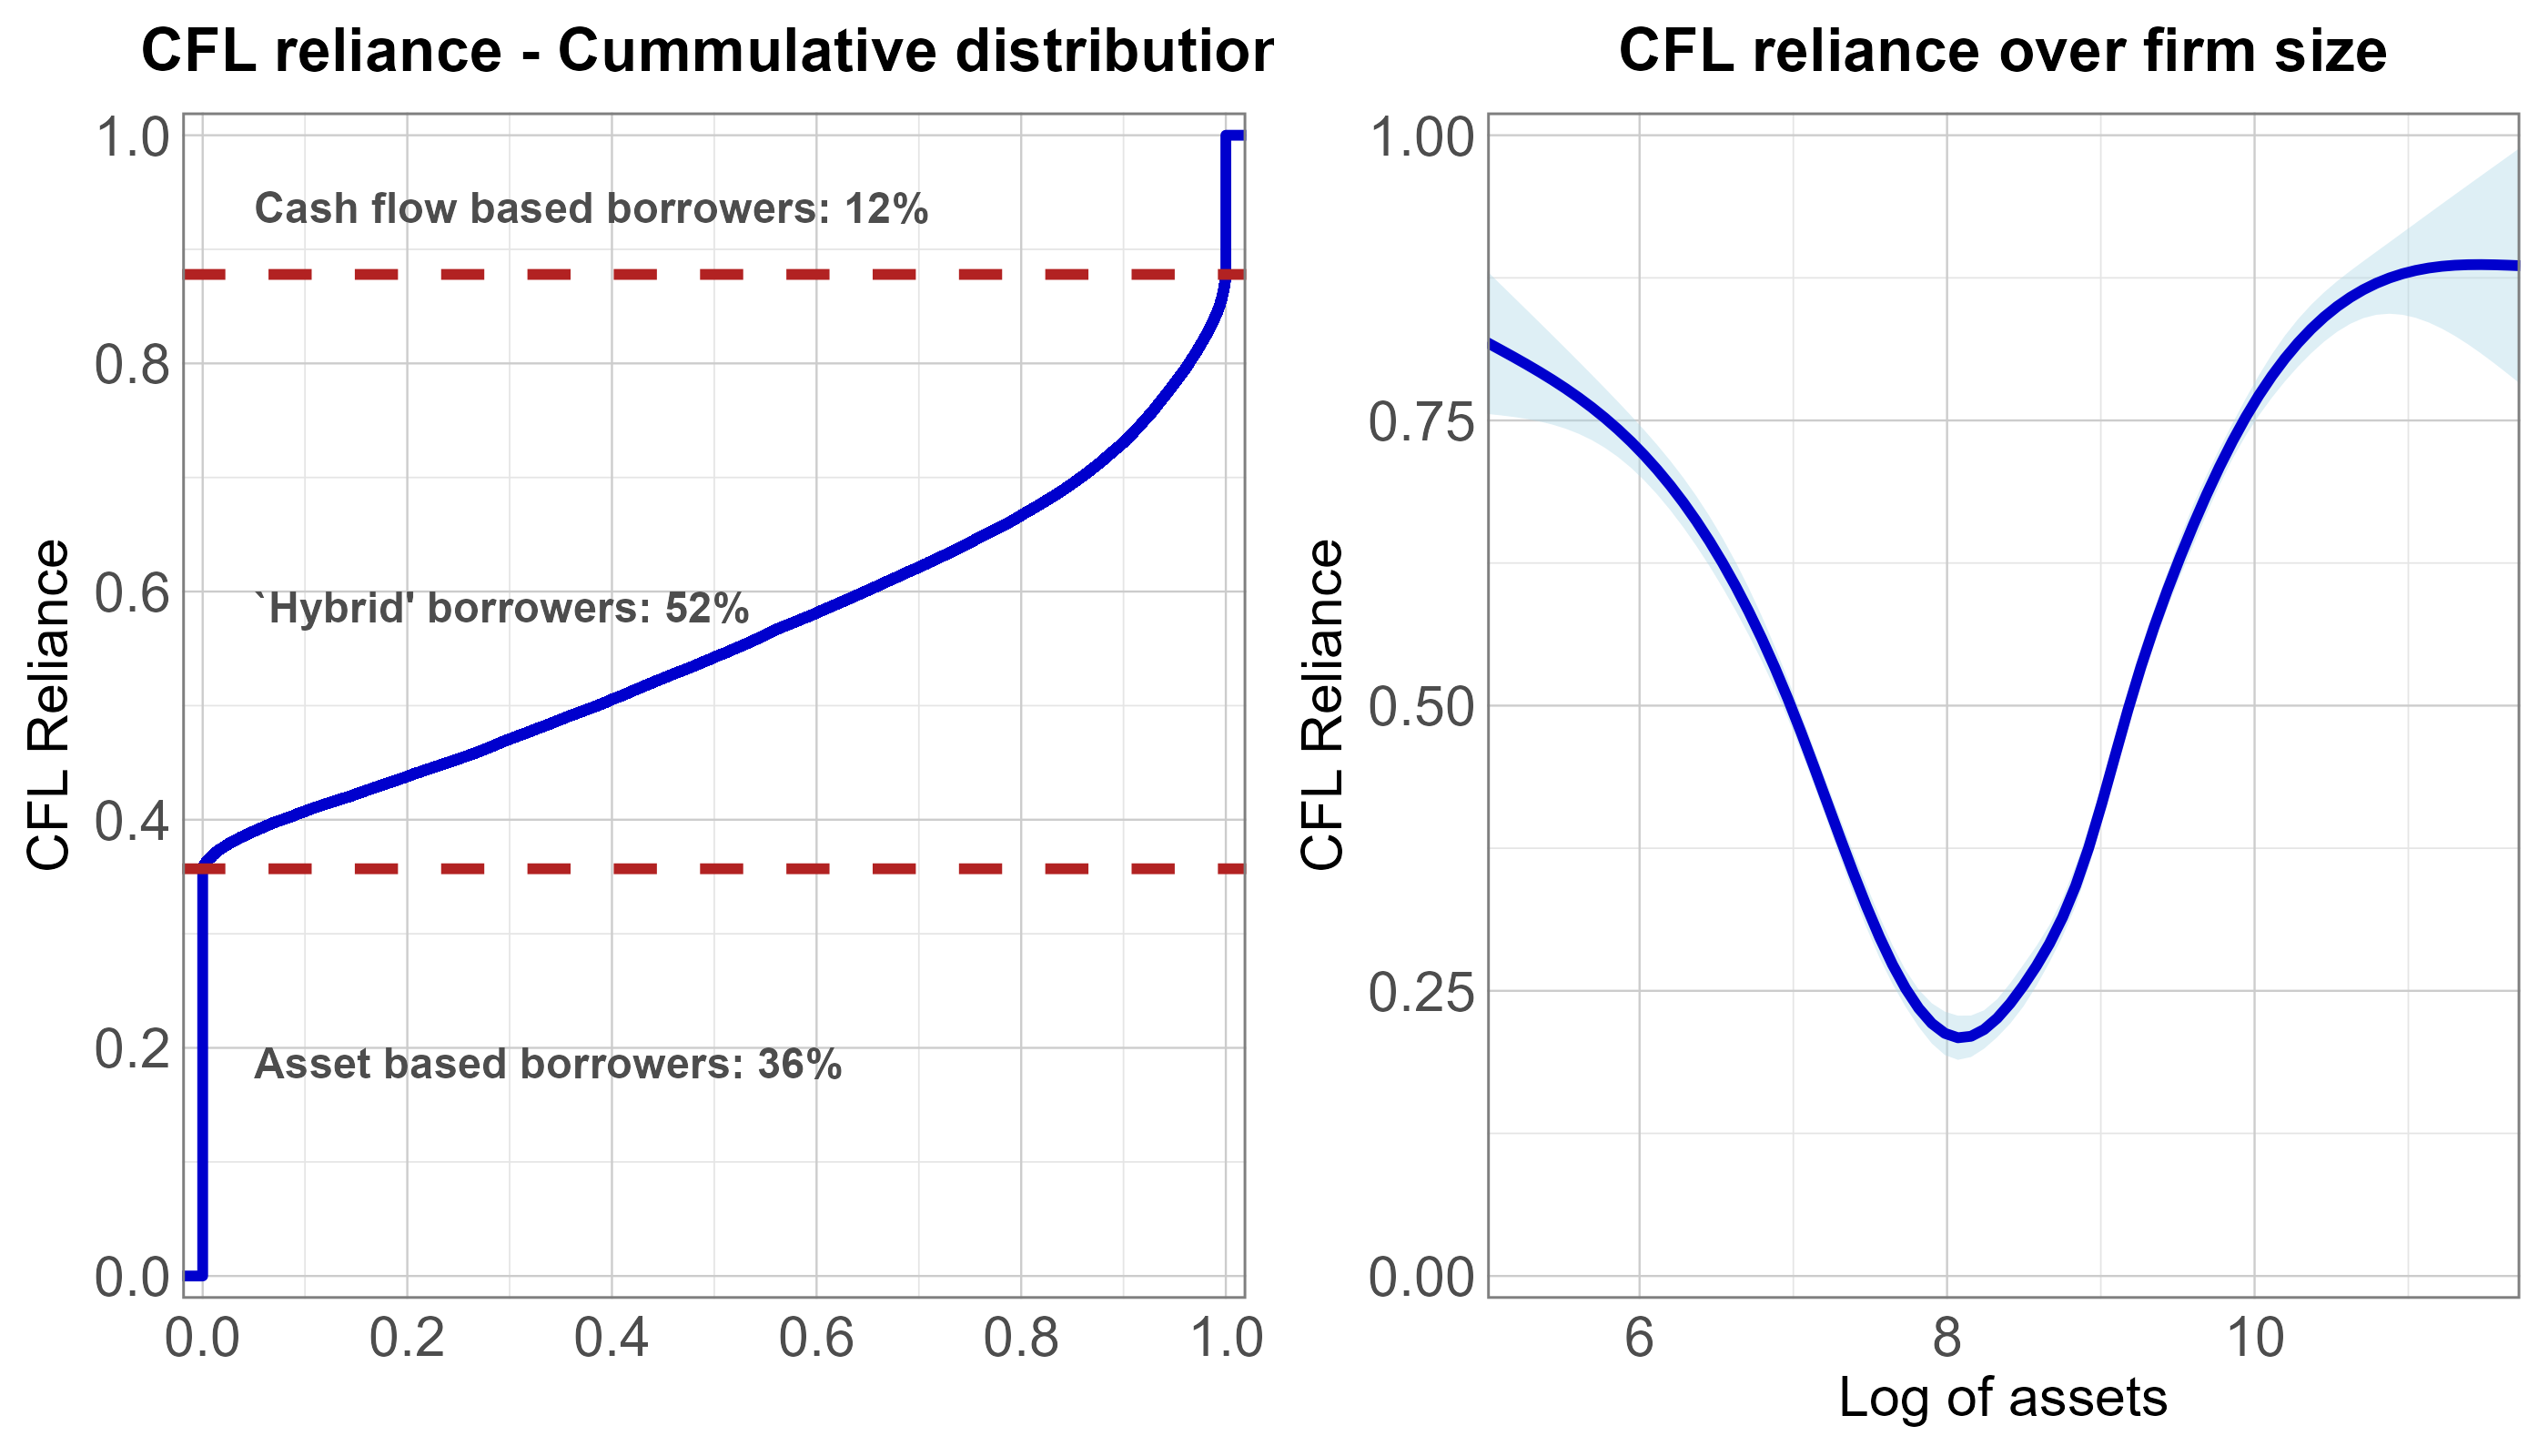
\includegraphics[width=1\textwidth]{C:/Users/szjud/OneDrive/Asztali gép/EBCs/CFL-git/Latex codes/Plots/smoothcfd.png}
\end{figure}
The multivariate analysis suggests that the most important predictors of CFL reliance include size (measured by the logarithm of assets), leverage, and the share of collateralizable assets on the balance sheet: more indebted firms become more likely to obtain CF-based finance, while a greater proportion of collateralizable assets is associated with lower CFL reliance. As I argue later, these variables are important in their own right, but they are also matter as determinants of the liquidation probability. Moreover, I include the square of the logarithm of assets in the regression. The coefficient for this variable is consistently positive and statistically significant in each regression, indicating the robustness of the U-shaped relationship in the multivariate setting. 

\subsection*{Structural model of debt financing strategies}
I study the debt financing decisions in a general equilibrium model that incorporates a representative household, heterogeneous firms (borrowers) and a competitive lender. Firms own capital and may borrow or save. The competitive lender co-finances investments into capital, subject to a zero-profit condition. Hence, the terms of borrowing are shaped by lenders' costs and payoffs under each type of debt contract. Cash flow-based contracts allow the lender to retrieve a share of the going-concern value of the firm in financial distress. On the other hand, asset-based contracts allow lenders to extract the liquidation value of firms. Hence, the terms of credit reflect lenders' expectation regarding the likelihood of liquidation for the particular firm.

To obtain results, I contrast a version of the model with asset-based lending only, to the model where firms can flexibly choose their reliance on CF-based borrowing. I find that the availability of CF-based borrowing makes the largest difference for small firms that lack the adequate capital stock to borrow against assets. Small but productive firms enter in greater numbers and reach their efficient size faster, which yields higher average productivity. The expected liquidation probability in this exercise is the function of size, and it is calibrated externally. I find that firms can obtain CF-based financing even if their liquidation probability is relatively high (around 70\%). I also explore alternative calibrations where small firms face an increased likelihood of liquidation. Facing higher ex-ante liquidation probability, most of these small yet productive firms lose access to cash flow-based financing. This underscores the importance of bankruptcy frameworks that encourage the reorganization of small firms.


\subsection*{Conclusion}

Despite the profound implications of cash flow-based (CF-based) debt contracts for macro-finance models, the motivations behind choosing this form of debt financing remain understudied. This paper examines the tradeoffs that govern firms' and lenders' decisions in this regard. In particular, I highlight the ex-ante probability of liquidation under financial distress as an important determinant of borrowing against future cash flows. Based on this analysis, I argue that bankruptcy frameworks should invest additional effort into incentivizing reorganization, particularly for small firms, since these corporations stand to benefit most from CF-based borrowing - but high liquidation probabilities may deprive them of this type of debt financing.

%\bibliographystyle{apalike} % Choose your desired bibliography style

%\begin{thebibliography}{99}
%\bibitem{drechsel2023} Drechsel, T. (2023). Earnings-based borrowing constraints and macroeconomic fluctuations. \textit{American Economic Journal: Macroeconomics}, \textbf{15}(2), 1-34.

%\bibitem{lian2021} Lian, C., \& Ma, Y. (2021). Anatomy of corporate borrowing constraints. \textit{The Quarterly Journal of Economics}, \textbf{136}(1), 229-291.

%\end{thebibliography}


\end{document}


